\section{Validation of the two-dimensional measurement}
\label{sec:validation}

In a simulated experiment, \emph{truth} is the known target distribution,
the \emph{prior} is the starting simulated truth distribution, and the
\emph{response} describes reconstruction and selection conditional on truth.
A closure test compares the unfolded estimate with its known target under a
specified deformation. Bias is the mean estimate minus that target over
repeated experiments; a single closure residual also contains sampling
fluctuations. Coverage is the fraction of repeated intervals containing the
specified truth, and tests the estimator and interval procedure together.
Table~\ref{tab:validation-questions} separates these questions before the
results. Repeating a numerical calculation checks neither interval calibration
nor the adequacy of the physical model.

\begin{table}[H]
\centering\footnotesize
\begin{tabular}{@{}p{0.16\textwidth}p{0.27\textwidth}p{0.25\textwidth}p{0.23\textwidth}@{}}
\toprule
Check & Target and estimator & Sample relation / measured quantity & Rule and conclusion \\
\midrule
Injected closure & Reweighted simulated truth; 1A LightGBM, five iterations & Same simulated response; residual under named truth or hidden-variable deformation & Thresholds below; passes depend on deformation and amplitude \\
\addlinespace
Miss completeness & Full truth inventory; production event mapping & Same event keys; truth-only entries retained & Membership and completeness invariants; no recovery or coverage claim \\
\addlinespace
Iteration stability & Same data; five versus ten iterations & Shared sample; movement of total and shape & Small observed movement; not a known-truth accuracy test \\
\addlinespace
Fixed-truth coverage & Fixed unfluctuated MC truth; LightGBM statistical estimator & Poisson pseudo-data; MC resampling shares the band's mechanism; pooled toy--bin containment & Predeclared coverage windows; earlier band fails. Rebuilt band awaits independent test \\
\bottomrule
\end{tabular}
\caption{Validation questions, targets and limits. Shared simulation is not an
independent detector-response test. Coverage pooled over bins is not a
simultaneous probability that every bin is covered.}
\label{tab:validation-questions}
\end{table}

\paragraph{Closure.}
Three existing closure families used playlist 1A, LightGBM and five iterations
(thresholds in parentheses).
% (1A lgbm 5-iter)
\begin{itemize}
  \item \textbf{Truth-reweight} (same factor for truth and reco weights):
        gaussian-$\pT$ residual \SI{0.046}{\percent}, tilt-$\pPar$
        \SI{0.013}{\percent} (thr \SI{1.5}{\percent}). Injected truth recovered.
  \item \textbf{Hidden-variable} (bias on $\Delta\pT=\pT^{\mathrm{reco}}-\pT^{\mathrm{truth}}$,
        a resolution variable outside the feature set): leakage linear in amplitude,
        $A=0.05/0.10/0.30\to0.57/1.14/3.43\,\%$ (thr \SI{3.0}{\percent});
        the first two amplitudes pass; the deliberately large $A=0.30$ arm exceeds
        the threshold.
  \item \textbf{Alt-model} (train on CV, pseudo-data from an alternative universe):
        MaCCQE \SI{0.068}{\percent}, Flux \SI{0.376}{\percent} (thr \SI{2.0}{\percent}).
\end{itemize}

\paragraph{Injected-feature recovery.}
The 2D gaussian-bump truth-reweight closure passes the unbinned-unfolding guide's
recovery test~\cite{Canelli:2025guide}. In the feature bins, the residual from injected truth is
\SI{1.69}{\percent} for an injected \SI{17.2}{\percent} feature
(ratio $0.098$), or $\approx10\times$ smaller. Recovery of the data's deviation
from the prior must leave a residual far smaller than the feature;
unfolding cannot manufacture discriminating power (3D: \S\ref{sec:3d-closure}).

The naive reco-vs-truth $\chi^2$ data-vs-prior test gives truth$>$reco.
As expected at high resolution, detector smearing lowers the
reco baseline and a stat-only diagonal omits unfolding covariance. The proper
full-covariance goodness-of-fit uses the $\chi^2$-vs-paper of
\S\ref{sec:results-tension} and the generator comparisons.

These closure tests validate the estimator; they are not used to assign a non-closure
uncertainty. Such an uncertainty would require a predeclared suite
of injection shapes and amplitudes rather than calibration to a single
Gaussian bump.

They do not test pseudo-data with a detector response that disagrees
with the unfolding response. Appendix~\ref{app:response-mismatch} defines a
complementary record-only $\Eavail$ response-mismatch closure and a more complete
leading-nucleon follow-up. No result from that test is claimed here.
\S\ref{sec:val-fiveaxis} validates the five-axis estimator, including background
subtraction.

\paragraph{What the remaining validation needs.}
The follow-up assessment~\cite{TwoDFollowup2026} distinguishes a proposed
split-sample width check from repeated-sampling coverage. With a fixed MC
bank, binning maps and purity correction, such a check can support only
conditional precision at its tested exposure; nonlinear unfolding does not
guarantee a simple half-to-full-exposure scaling. It cannot supply the
variation across independent MC populations. The original objective of
validated total uncertainties for all 205 bins, the integral and the
projections has no feasible route with the current inputs. It requires
independent populations or a validated generative law, a continuous
nuisance generator for total-interval tests, an untouched generator-truth
domain for bias checks, and the construction repairs in
\S\ref{sec:uq-2d-construction}. This is a limitation of the available
evidence, not a general impossibility result for 2D unfolding.

\subsection{Fixed-truth coverage of the 2D statistical band}
\label{sec:coverage}
This test asks whether the production 2D statistical band (\S\ref{sec:bootstrap}) covers a
\emph{fixed} truth at its nominal rate. Its design, criteria and positive control were
pre-registered before any toy ran (App.~\ref{app:provenance}, \texttt{coverage-fixed-truth}).

Each toy draws pseudo-data event by event as Poisson counts with means equal to the simulated
reconstructed weights. It resamples the simulation with the production Poisson(1) bootstrap, and
unfolds with the statistical band's estimator (lgbm, five iterations, fixed training seed), the
learner of the quoted central value at a different seed (\S\ref{sec:method-config}). The reference
$T$ is the unfluctuated simulated truth, identical in every toy. The no-fluctuation configuration
reproduces both the production closure output and $T$ exactly.

In reported bin $b$ of toy $t$, $z_{tb}=(U_{tb}-T_b)/(r_b T_b)$, where $r_b$ is the production
band's relative spread. Coverage $C_k$ is the fraction of all (toy, bin) pairs with $|z|\le k$,
with intervals from resampling whole toys. The band counts as nominal if its ratio to the true
scatter lies in $[0.9,1.1]$, which gives the windows $C_1\in[\covTwoDWinOneLo,\covTwoDWinOneHi]$
and $C_2\in[\covTwoDWinTwoLo,\covTwoDWinTwoHi]$. A FAIL at the interim look of 100 toys, with
99.5\% intervals, stops the study.

\textbf{The band fails: it undercovers in its tails.} At the interim look
($N_{\text{toy}}=\covTwoDNtoy$, 205 bins):
\begin{itemize}[nosep]
  \item $C_1=\covTwoDCOne$ $[\covTwoDCOneLo,\covTwoDCOneHi]$ is nominal (Gaussian 0.683).
  \item $C_2=\covTwoDCTwo$ $[\covTwoDCTwoLo,\covTwoDCTwoHi]$ lies entirely below its window
        (Gaussian 0.954).
  \item The pull RMS is $\covTwoDPullRMS$, and the mean pull is consistent with zero.
\end{itemize}
The pre-registered verdict is FAIL-undercoverage, and the study stopped by its futility rule. An
independent recomputation with its own code reproduces the pooled coverages, their intervals, the
controls and the secondary below.

The positive control rescales the band on the same toys. At $\times0.7$ and $\times1.3$, $C_2$
moves to $\covTwoDCTwoLowCtl$ and $\covTwoDCTwoHighCtl$, and both directions are flagged.

The failure is one of width, not bias. The per-bin pattern below is descriptive and post hoc.
\begin{itemize}[nosep]
  \item \textbf{Uneven in both directions.} The band is too wide in $\covTwoDNwide$ bins (pull RMS
        below 0.9) and too narrow in $\covTwoDNnarrow$ (above 1.1). The pooled $C_1$ is nominal
        partly through this cancellation; the median bin's pull RMS is $\covTwoDBinRMSmed$.
  \item \textbf{Where it is too narrow.} $\covTwoDNlowCTwo$ bins have a per-bin $C_2$ below 0.85.
        Of these, 21 form a block at $\pPar\ge\SI{15}{GeV/c}$ and $\pT<\SI{0.55}{GeV/c}$. Six more
        lie in the highest-$\pT$ row (\SIrange{2.5}{4.5}{GeV/c}) at $\pPar$
        \SIrange{6}{20}{GeV/c}. The $\covTwoDNedge$ bins with pull RMS above~2 carry
        \SI{\covTwoDDeficitShare}{\percent} of the $C_2$ deficit.
\end{itemize}

The band's replicas divide by a bootstrapped completeness that the central value (exactly~1)
does not carry. A secondary, added by amendment after the pilot, applies that division to the toys.
Scored against the same band, it overcovers: $C_1=\covTwoDRepCOne$, with its interval above the
window. By the rule fixed before the full run (its undercoverage branch was written after the
pilot pulls had been seen), the primary undercoverage is attributed to this term of the band's
construction. The attribution is partial: in the replica form, the $\pPar$
\SIrange{40}{60}{GeV/c} column still undercovers.
That term was removed on 2026-10-06 and the band rebuilt; the rebuilt band is the quoted one
(\texttt{KNOWN\_ISSUES.md} 84; App.~\ref{app:provenance}, \texttt{coverage-fixed-truth}). This
section's result is for the earlier band and was not re-tested.

\textbf{The rebuilt band, scored post hoc.} Rescoring the same 100 toys against the rebuilt band,
which is post hoc and partly circular (its MC part reuses the toys' resampling mechanism), removes
the tail undercoverage: $C_2=0.977$ $[0.974,0.980]$ and $C_1=0.781$ $[0.771,0.790]$, both above
their nominal windows, so the rebuilt band is wider than the toy scatter (pull RMS 0.84, mean pull
consistent with zero). The residual excess width lies in the data-statistics component: the
per-bin pull RMS falls as that component's share of the band's variance rises, which corresponds
to a data-statistics part about $1.6\times$ wider in $\sigma$ than the toys produce. Background
purity does not explain it. Its cause is not established. A post hoc bootstrap-on-one-toy
diagnostic, with a decision rule committed before it ran, is consistent with the closure toys
under-scattering, because their pseudo-data sit on the training MC events, rather than with the
data bootstrap over-scattering; it is neither an independent-population coverage test nor a
real-data calibration. The held-out-MC re-test that would separate the two is deferred until
after the publication package (\texttt{KNOWN\_ISSUES.md} 85). Split-sample width checks that
condition on the existing MC bank, binning maps and purity cannot establish repeated-sampling
coverage across independent populations, so validated total intervals over the full reporting
domain need new inputs as well as the construction repairs of \S\ref{sec:uq-2d-construction}.
% Source: state/ki84-rebuild-20261006/rescore_vl169_toys_vl170.json (vl170: C1 0.7806 [0.7709, 0.7902],
% C2 0.9769 [0.9737, 0.9800], pull_rms 0.843, pull_mean -0.027 [-0.058, 0.004]; label "POST HOC, DESCRIPTIVE";
% commit 5aab2d6d); KNOWN_ISSUES.md 85 (the 1.6x, the f-share regression, purity median 0.975);
% DECISION-RULE-20261006-ki85-bootstrap-diagnostic.md (outcome (b)); diagnostic 8eb40e5f. Moved here from the
% article on 2026-10-11, when its 2D-coverage subsection was shortened.

\textbf{Scope.} The result concerns the statistical band only.
\begin{itemize}[nosep]
  \item It changes no central value or quoted uncertainty.
  \item It tests the LightGBM statistical estimator at the band's training seed (seed~1), not at
        the quoted central value's seed~42.
  \item It says nothing about systematic, total or five-dimensional coverage.
  \item Its simulation-side scatter reuses the resampling that built the band, so only the
        data-side fluctuation is tested by an independent mechanism.
  \item Because $T$ equals the prior, it cannot detect regularization bias toward the prior.
\end{itemize}

\subsection{Other validation diagnostics}
\label{sec:val-other}

\paragraph{Unbinned diagnostic (C2ST).}
The classifier two-sample test (C2ST) AUC drops from $\approx0.535$ before
unfolding to $\approx0.501$ after, indicating removal of the reconstructed
data\,$\leftrightarrow$\,MC mismatch. A classifier is trained to separate the data from the
(reweighted) simulation in the full unbinned feature space, and its held-out AUC/accuracy is
compared to the chance value $0.5$. This binning-free check is strictly
\emph{descriptive}; we do \emph{not} quote a calibrated $p$-value. The C2ST as run
trains and evaluates on the same sample without cross-fitting. A valid null
would require re-running the full cross-fitted OmniFold pipeline per
pseudoexperiment. Calibrated unbinned goodness-of-fit remains
open~\cite{Canelli:2025guide}.

\paragraph{Same-ensemble pull diagnostic (not a coverage test).}
An earlier ensemble contains $N_{\text{toy}}=200$ 2D closure unfolds
(App.~\ref{app:provenance}, \texttt{coverage-toys}),
% (\texttt{sbatch\_coverage\_toys\_MEFHC\_200.sh}; rollup
% \texttt{uq/coverage\_toys.py}, summary \texttt{uq/coverage/coverage\_summary.txt})
with weighted MC reco pseudo-data and truth marginals stored in truth
histograms. Each uses its own bootstrap seed $k$ and per-event Poisson(1) draws,
as in production; seeds avoid collisions with production replicas.
% CLI: \texttt{-{}-closure} with \texttt{-{}-bootstrap-seed $k$}; truth histogram \texttt{hTruthXSec2D}
Toy seeds are independent; bins within a toy are correlated. The MC bootstrap
multiplies the truth weight, fluctuating both the unfolded result and stored truth.
% truth weight: \texttt{w\_truth}; stored truth: \texttt{hTruthXSec2D}
Stored truth varies in all 205 reported bins, so its all-toy mean
$\bar X^{\text{truth}}$ is not an independent fixed truth for a split-sample
coverage claim; it only centers a same-ensemble diagnostic.

In reported bin $i$ with $\bar X^{\text{truth}}_{i}>0$, define the across-toy
standard deviation $\sigma_{i}$ (ddof $=1$) and standardized residual
$r^{(t)}_{i}=(U^{(t)}_{i}-\bar X^{\text{truth}}_{i})/\sigma_{i}$.
Compare the per-bin fraction $c_{i}$ of toys with $|r^{(t)}_{i}|\le1$ to the unit-normal
$\Phi(1)-\Phi(-1)=\mathrm{erf}(1/\sqrt 2)\approx0.6827$ and the mean absolute
pull $\langle|r|\rangle$ to $\sqrt{2/\pi}$. The fraction with $|r|\le1$ is
\SI{\pullFrac}{\percent} (Gaussian reference $68.27\%$; $\Delta = +0.44\%$;
median $68.50\%$); $\langle|r|\rangle=\pullMeanAbs$ vs
$\sqrt{2/\pi}=\pullGauss$ (within $0.5\%$); the signed residual mean is
$+0.006 \pm 0.082\,\sigma$ (no bias); and \SI{97.6}{\percent} of bins have a
within-bin fraction above \SI{65}{\percent} (only $5$ of $205$ fall below).
These show that the standardized toy residuals are approximately normal.

With $\sigma_i$ estimated from the scored toys, these diagnostics are not a
frequentist coverage measurement and do not certify the bootstrap band. The figures
serve only as standardized-pull/Gaussianity diagnostics; no coverage number is quoted from
this ensemble. The fixed-truth test above is the 2D coverage statement (App.~\ref{app:history}).

\paragraph{Stability and efficiency.}
The 5-iter total $\sigma$ is within \SI{0.026}{\percent} of 10-iter (per-bin shape RMS
\SI{1.54}{\percent}); HistGBT and exact-GBT agree on total $\sigma$ to
\SI{0.04}{\percent} (both measured for the exact-split cross-check). Efficiency (Fig.~\ref{fig:eff}) reproduces the published
Fig.~5.

\begin{figure}[H]
  \centering
  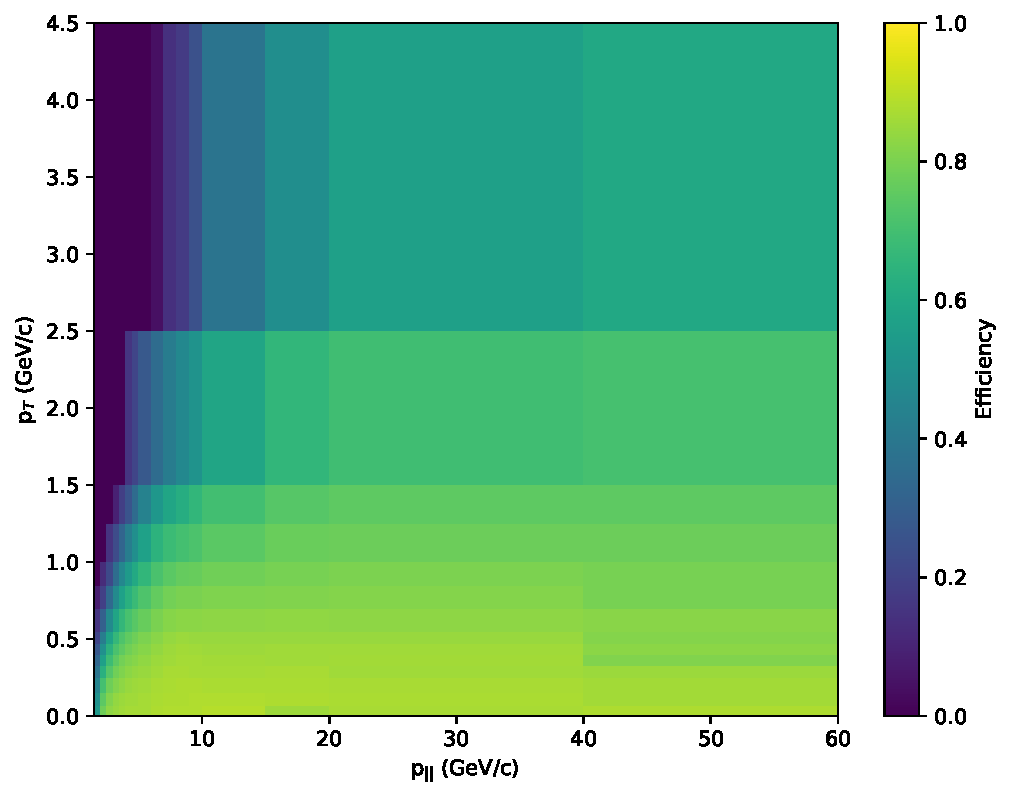
\includegraphics[width=0.62\textwidth]{MEFHC_5iter_xsec_eff_heatmap}
  \caption{Selection efficiency on the $(\pT,\pPar)$ truth grid. Efficiency is
  diagnostic only; OmniFold's miss treatment natively corrects acceptance
  (\S\ref{sec:method-algo}).}
  \label{fig:eff}
\end{figure}
